\documentclass[12pt]{article}
\usepackage[spanish, english, es-tabla]{babel}
\usepackage[utf8]{inputenc}
\usepackage{amsmath,amssymb}
\usepackage{graphicx}

\usepackage{array}

% text font 

\usepackage{courier}

%\usepackage{fontspec}

\usepackage[dvipsnames]{xcolor}

\usepackage{hyperref}
\usepackage{subcaption}
\usepackage[left = 2cm, right = 2cm, bottom = 2cm, top = 3cm]{geometry}

\hypersetup{
	colorlinks=true,
	linkcolor=black,
	%filecolor=magenta,      
	urlcolor=cyan,
}

\hypersetup{
	pdftitle= {Diseño y automatización de sistema de alimentación para animales a través de la tecnología LoRa},
	pdfauthor = {Lucía Francoso Fernández},
	pdfsubject = {Electrónica y comunicaciones móviles},
	pdfkeywords = {Arduino, LoRa, automatización, LoRaWAN, punto a punto, OpenSource}
}

% https://tex.stackexchange.com/questions/60209/how-to-add-an-extra-level-of-sections-with-headings-below-subsubsection
\newcommand{\subsubsubsection}[1]{\paragraph{#1}\mbox{}\\}
\setcounter{secnumdepth}{4}
\setcounter{tocdepth}{4}

\begin{document}
	\selectlanguage{spanish}

	\title{Diseño y automatización de sistema de alimentación para animales a través de la tecnología LoRa}
	\author{Lucía Francoso Fernández}
	\date{Marzo 2021}
	
	\maketitle
	\pagebreak
	
	\tableofcontents
	
	\pagebreak

	\listoffigures
	\addcontentsline{toc}{section}{Índice de figuras}

	\listoftables
	\addcontentsline{toc}{section}{Índice de tablas}
	
	\section[Introducción]{Introducción} %corchetes, marcapaginas, llaves, texto
	
	Tras finalizar los estudios de grado en ingeniería en sistemas de telecomunicaciones, se requiere como último paso para la obtención del título la elaboración del \textit{Trabajo Fin de Grado} (TFG). 
	El TFG como tal tiene unos objetivos claros, los cuales son demostrar que se han adquirido las competencias básicas intrínsecas al grado, y que el alumno es capaz de seguir aprendiendo a partir de los conocimientos ya obtenidos, innovar, desenvolverse ante un problema determinado y, en resumen, saber llevar a cabo una investigación o proyecto que tenga como objetivo la resolución de dicho problema. \\
	
	\noindent En este documento, se recoge el proyecto realizado como TFG,  el cual va en línea con la filosofía y objetivos del \textit{Trabajo Fin de Grado} en sí mismo. Se detallará el proceso de creación de un sistema de alimentación para animales automatizado, donde se monitorizan de manera remota el estado de los tanques de reserva de agua y pienso. Así, se pretende exponer el conjunto de elementos hardware y software que serán necesarios para monitorizar, automatizar y acceder a ciertos datos de forma remota empleando, principalmente, Arduino y LoRa.\\
	
	
	\subsection[Contexto y justificación del trabajo]{Contexto y justificación del trabajo}

	\noindent Este proyecto ha sido concebido con el objetivo principal de ayudar a la preservación de la vida animal, ante el aumento de especies en extinción, sobretodo en lo que llevamos de siglo \footnote{\href{https://www.nationalgeographic.com.es/naturaleza/grandes-reportajes/animales-peligro-extincion_12536}{National Geographic} , \href{https://www.bbc.com/mundo/noticias-54036796}{BBC}, \href{https://www.worldwildlife.org/descubre-wwf/historias/que-significa-especie-en-peligro-de-extincion}{WWF}, \href{https://www.fundacionaquae.org/causas-perdida-biodiversidad/}{Fundación AQUAE}}, y ante el hecho de que miles de animales domésticos siguen siendo abandonados al año en España \footnotemark. \\
	
	%Fundación Affinity, 20 minutos, La Razón, RTVE
	\footnotetext{\href{https://www.fundacion-affinity.org/observatorio/infografia-el-nunca-lo-haria-estudio-de-abandono-y-adopcion-2020}{Fundación Affinity}, \href{https://www.20minutos.es/noticia/4318383/0/el-abandono-animal-en-espana-aumenta-un-25-en-las-ultimas-semanas/}{20 minutos}, \href{https://www.larazon.es/medio-ambiente/20201118/qxv6yuokargfbnjvknn6bhm4ze.html}{La Razón}, \href{https://www.rtve.es/noticias/20200608/abandonos-animales-domesticos-se-han-disparado-espana-durante-meses-confinamiento/2015761.shtml}{RTVE}}

	\noindent Es por ello que se requiere de ayuda activa para paliar estos problemas. Las tareas de carácter solidario, en bastantes casos, no siempre cuentan con suficientes voluntarios; además, siendo un problema tan extendido y avanzado, el número de acciones que hay que llevar a cabo para aliviarlo es alto para un número limitado de voluntarios, los cuales deben incrementar considerablemente el tiempo que pasan realizando este tipo de tareas. 
	Tanto si se trata de un refugio de animales domésticos abandonados, como de reservas naturales donde se intenta repoblar una especie, los animales dependen enteramente del trabajo de los voluntarios. Así pues, es de vital importancia la optimización de las tareas de voluntariado, su automatización e, incluso, control remoto, mediante la creación de herramientas que ayuden a reducir el tiempo que se destina a tareas rutinarias para poder utilizar ese tiempo a otras tareas (de rescate, o de financiación para el mantenimiento de las instalaciones y de los propios animales, por ejemplo). \\
	
	\noindent Con el objetivo en mente de ayudar a la preservación de la fauna (y con ello, de la vida de los ecosistemas terrestres), evitando la extinción de especies y el abandono animal, se ha concebido y desarrollado este proyecto teniendo en cuenta los diferentes casos de uso (emplazamientos donde se podrá instalar el sistema, características del entorno), mejor adaptación a ellos, relación entre buenas prestaciones y bajo consumo, precio total del producto, o facilidad de uso por parte de un usuario medio. Es por ello que desde el principio se propone una serie de actuaciones a realizar, acorde a lo anteriormente mencionado, tales como:
	
	\begin{itemize}
		\item El diseño del sistema de alimentación será tal que el producto final pueda ser instalado no sólo en hogares, sino en sitios remotos, donde el acceso a recursos tales como la electricidad o Internet son escasos o inexistentes. Así pues, el dispositivo utilizará energía solar y baterías recargables, comunicación de bajo consumo y largo alcance y modo de ahorro de energía. 
		\item El dispositivo final no será pesado ni voluminoso, facilitando así tanto su transporte como su manejo. No dejará al alcance del animal electrónica, de manera que evitaremos que los animales estén en contacto con ella y posibles problemas de humedad presente en el entorno; se usarán protecciones adecuadas a la calidad de los componentes del dispositivo.
		\item El dispositivo contará con una pantalla OLED que permitirá ver a la persona que esté físicamente delante de él si funciona correctamente. También se permitirá el acceso a datos a personas interesadas que quieran consultarlos de manera remota.

	\end{itemize}

	
	\subsubsection[Ejemplo de caso de aplicación]{Ejemplo de caso de aplicación}
	
	Un ejemplo de caso de aplicación sería el entorno donde se desea situar uno de estos dispositivos para validar su funcionamiento, que en este caso se trata del refugio perteneciente a la protectora Patitas Unidas Los Alcázares, situado en el término municipal de Torre Pacheco (Murcia).
	La elección de esta ubicación se fundamenta en una serie de razones:
	
	\begin{itemize}
		\item Al ser voluntaria para esta protectora, conozco bien sus necesidades, es decir, qué puede ser de utilidad para la protectora en el refugio y qué soluciones se han probado para determinados problemas que han ido surgiendo; además, conozco bajo qué condiciones climáticas es vulnerable y qué necesidades esporádicas emergen bajo dichas condiciones. Teniendo en cuenta la zona geográfica donde se ubica (Murcia), y los años de experiencia en el refugio, se ha detectado una problemática que se manifiesta durante  periodos continuados de lluvias (lluvias torrenciales, DANA, gota fría), la cual consiste en la inundación de las zonas colindantes al refugio, inclusive carreteras de acceso, lo que impide llegar a él (cierre de carreteras, niveles altos de riesgo por precipitación, o el simple hecho de contar con grandes volúmenes de agua en la carretera que impiden la circulación segura por la vía). De
		\item Se trata de un entorno sin electricidad y sin internet. Desarrollar un proyecto y probarlo en este tipo de entorno nos ayudará a la hora de extrapolarlo a otros emplazamientos donde la ausencia de este tipo de recursos supone también una limitación y un aspecto a tener en cuenta para definir y desarrollar el proyecto en sí mismo.
		\item Se puede intentar establecer un enlace punto a punto, ya que se puede dejar fijo un equipo transmitiendo o recibiendo que, además, se conecte a internet (ya que es un recurso disponible) para subir los datos que reciba del otro extremo. Un equipo estará presente en el refugio y el otro en una casa con internet y electricidad; esto significa que al menos este extremo será más controlable, y será este extremo el que subirá datos a la nube. Nos tendremos que preocupar más del otro extremo, donde no tendremos electricidad ni internet y donde situaremos los sensores que recogerán datos y realizarán la automatización.
	\end{itemize}
	
	\subsection[Objetivos del trabajo]{Objetivos del trabajo}
	
	El objetivo fundamental del presente trabajo es el diseño de un sistema de alimentación para animales que permita la monitorización de los niveles de agua y pienso que se encuentran en depósitos de reserva, los cuales rellenan un bebedero y un comedero, respectivamente.  Con ello, se pretende automatizar el proceso de alimentación de animales, además del uso de la tecnología LoRa para tener acceso al estado del sistema de forma remota. Así pues, los objetivos concretos son:
	
	\begin{itemize}
		\item Realizar una aproximación a la tecnología LoRa.
		\item Diseñar el sistema de alimentación para animales.
		\item Realizar tanto simulaciones para el enlace LoRa que se creará entre transmisor y receptor, como cálculos teóricos que determinen si el enlace es posible.
		\item Construir el prototipo y probarlo en entorno controlado y, posteriormente, en entorno real.
		\item Crear una plataforma de representación de datos.
	\end{itemize}
	
	\subsection[Enfoque y método seguido]{Enfoque y método seguido}
	\subsection[Planificación del trabajo]{Planificación del trabajo}
	\subsubsection[Alcance]{Alcance}
	\subsubsection[Hitos]{Hitos}	
	\subsubsection[Calendario de trabajo]{Calendario de trabajo}
	\subsubsection[Tareas y diagrama de Gantt]{Tareas y diagrama de Gantt}
	\subsubsection[Riesgos e incidencias]{Riesgos e incidencias}
	\subsubsection[Recursos]{Recursos}
	\subsection[Breve sumario de productos obtenidos]{Breve sumario de productos obtenidos}
	\subsection[Breve descripción de los capítulos restantes de la memoria]{Breve descripción de los capítulos restantes de la memoria}
	
	\pagebreak
	

	\section[Estado del arte]{Estado del arte}  
	
	\noindent En este capítulo se va a exponer un análisis del estado del arte relativo al proyecto (tecnologías y técnicas necesarias para el diseño del sistema planteado). Este análisis se centra en la situación actual en tanto a  la automatización del proceso de alimentación de animales, técnicas, sistemas y proyectos similares y conceptos introductorios a Arduino y LoRa, fundamentales para poder materializar este proyecto.
	
	\subsection[Contexto actual]{Contexto actual}
	
		\noindent Existen muchos proyectos Open Source relacionados con la alimentación automática o semiautomática de animales domésticos, principalmente gatos y perros. Sin embargo, no existen proyectos que usen LoRa como tecnología radio, sino que emplean la red local WiFi del hogar donde se sitúe el dispositivo de alimentación.
	
	\noindent A pesar de ello, se ha visualizado este tipo de proyectos y tenido en cuenta para el desarrollo del prototipo en tanto a apariencia externa, comodidad de uso, eficiencia de los componentes, o, incluso, opciones para mover el pienso desde la reserva hasta el comedero del animal, o el agua desde la reserva hasta el bebedero.
	
	\subsection[Trabajos relacionados]{Trabajos relacionados}
	

	
	\subsection[Resumen del capítulo]{Resumen del capítulo}
	
	\pagebreak
	
	\section[Diseño del sistema]{Diseño del sistema}
	
	\noindent A lo largo de este capítulo se procede a desglosar el \textcolor{RubineRed}{\texttt{diseño del sistema}}, exponiendo las tecnologías y los dispositivos que se van a emplear tanto en monitorización como en comunicaciones. Por tanto, tras realizar una pequeña introducción de las tecnologías necesarias en el diseño, se procede empleando una metodología en cascada que vaya presentando a cada paso los subsistemas finalizados y completamente operativos.
	
	\subsection[Funcionalidades a cubrir]{Funcionalidades a cubrir}
	
	\noindent Teniendo claros los objetivos que se persiguen con este proyecto, el siguiente paso es definir las funcionalidades que ofrecería el sistema global que se pretende crear, ya que a partir de esta definición podremos empezar a deducir y establecer qué componentes son necesarios para llevar a cabo dichas funcionalidades. \\
	
	\noindent Definimos 3 funcionalidades: \\
	
	\begin{enumerate}
		\item Alimentación del dispositivo autónoma
		\item Automatización y monitorización (I): bloque microcontrolador
		\item Automatización y monitorización (II): bloque comunicación radio 
		\item Automatización y monitorización (III): bloque comedero (sensores, actuadores)
		\item Automatización y monitorización (IV): bloque bebedero (sensores, actuadores)
		\item Integridad mediante prototipo exterior
	\end{enumerate}
	
	\subsection[Búsqueda soluciones]{Búsqueda de soluciones para cada funcionalidad}

	\subsubsection{Alimentación autónoma del dispositivo}
	\noindent Se entiende por alimentación autónoma la obtención de energía suficiente para el correcto funcionamiento de un dispositivo o un sistema, y que dicha obtención de energía se realice de manera cíclica e independiente o prácticamente independiente, es decir, no dependa de la acción y supervisión constante de una persona. \\
	
	\noindent Para determinar la forma en la que alimentaremos nuestro proyecto, es imprescindible conocer bien las necesidades energéticas que lo limitarán; hay que determinar, por tanto, el consumo estimado de los componentes que conforman el proyecto. También es importante saber el tamaño y/o el destino de nuestro proyecto, para determinar si estará limitado a la hora de su transporte por una fuente de alimentación pesada, o si esta no limita en absoluto; será fundamental, además, conocer la ubicación de nuestro proyecto, es decir, si estará en el exterior o interior, si el ambiente será excesivamente frío, cálido o húmedo.\\
	
	\noindent A continuación, se mencionarán algunas soluciones para alimentación autónoma. Primero, se realizará una introducción teórica a términos y definiciones que nos permitan entender su funcionamiento; después, se presentarán opciones dentro de la categoría, haciendo énfasis en sus ventajas y desventajas, y anotando para qué proyectos es recomendable su uso. Por último, se pueden mostrar datos comparativos entre las opciones dentro de la categoría para una mejor visualización de dichas diferencias.\\ 
	
	\noindent \textbf{Baterías recargables} \\
	
	\noindent \textit{Términos y definiciones} \\
	
	\noindent Las características eléctricas de una batería definen cómo actuará en el circuito, y las características físicas tendrán un enorme impacto en el tamaño y peso global del producto al que va a alimentar. \\
	\noindent Es por ello que, a la hora de escoger una batería, hay que tener presente los requerimientos de alimentación del proyecto, ya que ésta debe ser capaz de suministrar suficiente energía para que funcione correctamente. Algunos parámetros que hay que comprobar son las tensiones mínima y máxima que otorga, la corriente, la capacidad y el material del que está hecha la batería. \\
	
	\noindent Se presenta, a continuación, una lista más extensa y explicada de los parámetros más importantes de las baterías: 
	
	\begin{itemize}
		\item  Una \textit{\textbf{celda}} es un dispositivo electroquímico capaz de suministrar la energía que resulta de una reacción química interna a un circuito eléctrico externo. \\
		Una batería se compone de una o más celdas, conectadas en paralelo o en serie para obtener la capacidad de corriente/voltaje requerida (las baterías compuestas por celdas conectadas en serie son las más comunes).
		\item La \textit{\textbf{resistencia en serie equivalente (ESR)}} es la resistencia interna presente en cualquier celda que limita la cantidad de corriente máxima que puede entregar.
		\item La \textit{\textbf{capacidad}}, medida en amperio-hora (Ah), de una batería (o celda) es su figura de mérito más importante: se define como la cantidad de corriente que una batería puede entregar durante 1 hora antes de que el voltaje de la batería llegue al final de su vida útil. 
 		\item La \textit{\textbf{tasa ``c''}}  es una corriente que es numéricamente igual a la clasificación Ah de la celda. Las corrientes de carga y descarga se expresan típicamente en fracciones o múltiplos de la tasa c. 
 		\item El \textit{\textbf{MPV (voltaje de punto medio)}} es el voltaje nominal de la celda y es el voltaje que se mide cuando la batería se ha descargado el 50\% de su energía total. \\
 		\noindent La oscilación de voltaje máxima y mínima del valor nominal es una consideración de diseño importante: una curva de descarga "más plana" significa menos variación de voltaje que el diseño debe tolerar.
 		\item El \textit{\textbf{voltaje de celda medido al final de su vida útil}} se llama \textit{\textbf{EODV}}, que significa \textit{Fin de voltaje de descarga} (algunos fabricantes se refieren a esto como \textit{EOL} o \textit{voltaje de fin de vida útil}). \\
 		\noindent Cuando se carga al máximo, el voltaje real de la celda será más alto que el MPV. Al acercarse al punto EODV (final del voltaje de descarga), el voltaje de la celda será menor que el MPV. 
 		\item La \textit{\textbf{densidad de energía gravimétrica}} de una batería es una medida de cuánta energía contiene una batería en comparación con su peso. Normalmente viene expresada en Watt-horas/kilogramo (Wh/kg).
 		\item La \textit{\textbf{densidad de energía volumétrica}} de una batería es una medida de cuánta energía contiene una batería en comparación con su volumen. Normalmente se expresa en Watt-horas/litro (Wh/l)
 		\item Un \textit{\textbf{cargador de voltaje constante}} es un circuito que recarga una batería obteniendo solo la corriente suficiente para forzar el voltaje de la batería a un valor fijo.
 		\item Un \textit{\textbf{cargador de corriente constante}} es un circuito que carga una batería al suministrar una corriente fija a la batería, independientemente del voltaje de la batería.
	\end{itemize}

	\pagebreak
	
	\begin{figure}[h]
		\begin{center}
			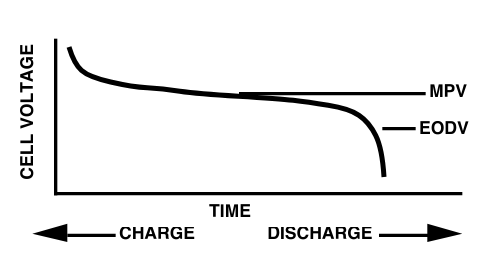
\includegraphics[width=0.7\textwidth]{img/chargeDischargeCurve_TxInst.png}
			\caption{Curva de la carga/descarga de una batería.}
		\end{center}
	\end{figure}

	\pagebreak
	
	% \noindent Entrarían dentro de esta categoría  las conocidas baterías recargables, formato LiPo o Li-ion, por ejemplo, o formato powerbank, que si bien en su interior usan baterías LiPo/Li-ion, el encapsulado en el que se presentan y la forma en que se usan son totalmente diferentes. \\
	
	\noindent \textit{Tipos de baterías recargables}\\
	
	\noindent Las principales baterías recargables que existen son: \\
	
	\begin{enumerate}
		
		\item \textit{Lithium polymer} (LiPo).  Son baterías de gran densidad de energía disponible, es decir, almacenan la mayor parte de energía para un determinado tamaño. Es por esta razón por la que los teléfonos móviles, los portátiles y otros dispositivos ligeros en peso usan baterías LiPo. Sin embargo, esta alta densidad de energía lleva consigo un coste/inconveniente, y es que son caras, y no son sólo las baterías en sí; cuando se trabaja con baterías de litio, hay que realizar una inversión para conseguir una circuitería especial que mantenga segura la batería. Por ejemplo, cuando estas cargando una batería LiPo, hay que asegurarse de que nunca se excedan los 4.2V por celda; las baterías LiPo explotarían si las sobrecargaras. No solo la carga de la batería es delicada, sino que la descarga también lo es; si se descarga una batería LiPo por debajo de 3V por celda, se perderá permanentemente parte de su capacidad, e incluso pueden deformarse/hincharse. Finalmente, hay que estar pendiente constantemente de la temperatura, para evitar que la batería se sobrecaliente. A pesar de todo esto, es común usar baterías LiPo en proyectos ligeros y pequeños, siempre y cuando se tenga un buen circuito de carga, un buen circuito de descarga (que proteja a valores bajos de tensión, haciendo de corte en el mínimo de tensión de la batería) y un buen circuito de monitorización de temperatura. 
		
		\item \textit{Lithium-ion} (Li-ion). Son muy similares a las baterías LiPo, pero a diferencia de estas, el electrodo negativo es líquido y el encapsulado y formato de presentación es totalmente diferente (las Li-ion suelen venderse sin protección y en apariencia son similares a unas pilas alcalinas AA). Una batería Li-ion almacena más potencia que las LiPo (mayor capacidad), ofrece mayores corrientes de descarga, es menos costosa de fabricar (y por tanto tienen un precio de venta más asequible),  y tiene un tiempo de vida más largo (aunque con el tiempo pierde sus propiedades). Es, al igual que las LiPo, inflamable si se daña, se calienta en exceso o se sobrecarga. El empaquetado más común es el 18650, y en el mercado existen circuitos de protección varios para evitar la sobrecarga y la sobredescarga  para este encapsulado en concreto, por lo que es una opción barata y sencilla para conseguir un prototipado rápido y realizar pruebas del mismo, siempre y cuando el proyecto no exija mucha potencia; si el proyecto exigiera más tensión de la que proporciona la batería, se puede considerar obtener más unidades y realizar una configuración en serie para aumentar la tensión, o en paralelo si lo que se desea es aumentar la capacidad (usando siempre un \textit{Battery Management System} o BMS, para mantener las baterías balanceadas entre sí). Esta opción se puede considerar para baterías LiPo, pero para usuarios principiantes o poco experimentados resultará, probablemente, más complejo.
		
		\item \textit{Lithium Iron Phosphate} (LiFePO4). Son similares a las baterías LiPo, con la salvedad de que no son propensas a explosiones, como lo pueden ser las LiPo, si no se manipulan correctamente o las condiciones anteriormente mencionadas no se dan. También requieren una apropiada circuitería para cargarlas y descargarlas con cuidado, y si se comete un error se perderá permanentemente parte de la capacidad de la batería. Además, son un poco más pesadas que las baterías LiPo. Se usan normalmente en robots ligeros, herramientas eléctricas y juguetes por radio control, ya que son baterías bastante buenas entregando grandes cantidades de energía en un factor de forma pequeño y liviano.
		
		\item \textit{Sealed lead-acid} (SLA). Son una opción si se quiere comprar una batería no muy costosa, a la vez de evitar enfrentarnos a circuitos de protección de la batería. Estas baterías son bastante más duraderas que una batería de litio, y también son mejores para hacer frente a sobrecargas accidentales o sobredescargas. Tienen una excelente relación calidad-precio y también son el mejor tipo de batería frente a temperaturas extremas; es por esta razón que las baterías de plomo (o ácido-plomo) son la opción estándar para coches, motos, almacenamiento de energía solar y fuentes de alimentación de emergencia. El inconveniente de usar baterías de plomo es que son grandes y pesadas. No es recomendable, por tanto, usar baterías de plomo en aplicaciones portátiles.
		
		\item Níquel-cadmio (\textit{Nickel-cadmium}, NiCd). Los dispositivos portátiles, como los primeros teléfonos móviles, usaban baterías de níquel-cadmio. Son baterías baratas, que en teoría duran más tiempo que las baterías SLA; sin embargo, sufren el llamado efecto memoria, por lo que hay que regularmente descargarlas por completo, luego recargarlas por completo para mantener una alta capacidad, ya que, de lo contrario, estaríamos perdiendo vida útil de la batería. Así pues, en la actualidad no se suele usar este tipo de baterías, aunque se siguen vendiendo.
		
		\item \textit{Nickel Metal Hydride} (NiMH). Las baterías de níquel-metalhidruro o de níquel hidruro metálico tienen una mayor densidad de energía que las baterías de níquel-cadmio, en tanto a precio no son mucho más costosas y no sufren el efecto memoria. Son más grandes y pesadas que las baterías de litio, pero es bastante seguro trabajar con ellas, por lo que son las baterías más usadas por el consumidor medio en términos de pilas recargables (las encontramos en cualquier supermercado, y cargarlas es barato y simple). Hay que tener en cuenta que las baterías de NiMH, por norma general, tienen un ratio de autodescarga elevado, lo que quiere decir que a pesar de que no se esté haciendo uso de la batería, se autodescargan igualmente en un par de meses, lo que hace que no sean una buena opción para objetos de uso cotidiano (como mandos a distancia). Se recomienda que, si se necesita hacer uso de este tipo de baterías, se adquieran con bajo ratio de autodescarga (como Panasonic Eneloop), las cuales pueden resultar más baratas a largo plazo que comprar unas pilas alcalinas.
		
	\end{enumerate}
	
	\noindent \textit{Comparativa entre tipos de baterías recargables} \\
	
	\noindent \textit{\textbf{Densidad de energía}}
	
		\begin{figure}[h]
		\begin{center}
			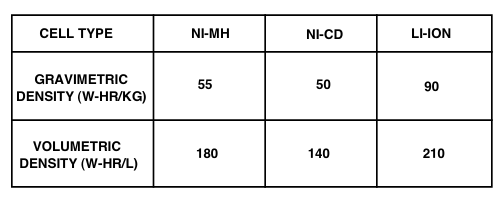
\includegraphics[width=0.7\textwidth]{img/energyDensityComparison_TxInst.png}
			\caption{Comparación densidad de energía para diferentes baterías.}
			\label{fig: comparación densidad energía}
		\end{center}
	\end{figure}
	
	\pagebreak 
	
	\noindent Al revisar los datos de la Figura \ref{fig: comparación densidad energía}, la ventaja de Li-Ion en densidad gravimétrica es claramente la más sorprendente, casi duplicando las cifras de Ni-Cd y Ni-MH. Esto significa que los productos que funcionan con celdas de iones de litio se pueden hacer mucho más livianos sin sacrificar el tiempo de ejecución. Alternativamente, si el peso de la batería se mantiene igual, el tiempo de funcionamiento se duplicará si se utilizan baterías de iones de litio. Este hecho explica la razón por la que Li-Ion está reemplazando rápidamente al Ni-MH en los teléfonos celulares y computadoras portátiles de primera línea. \\
	
	\noindent \textit{\textbf{Estabilidad de tensión o tensión de celda}}\\
	
	\noindent La tensión proporcionada para alimentar la carga es la más importante: las baterías Ni-Cd y Ni-MH tienen una tensión por celda de 1.25V (sus tensiones de descarga se asumen por norma general idénticas). \\
	\noindent La tensión por celda de las baterías Ni-Cd y Ni-MH son sólo una tercera parte de la tensión nominal de 3.6V proporcionada por una celda de Li-ion (Figura \ref{fig: curva descarga celdas}), lo que significa que se requerirían tres celdas de Ni-Cd/Ni-MH conectadas en serie para igualar la tensión de una única celda de Li-ion.\\
	\noindent Sin embargo, la Figura \ref{fig: curva descarga celdas} muestra también la gran ventaja de las baterías Ni-Cd y Ni-MH: su curva de descarga es extremadamente plana, próxima a la de una batería ideal. Esta importante diferencia entre tipos de baterias significa que las celdas de Ni-Cd y Ni-MH son adecuadas para su uso con reguladores lineales, pero las baterías de Li-ion requieren convertidores reductores (\textit{Buck converters}) para obtener una buena eficiencia de conversión de energía en la fuente de alimentación. \\
		
	\begin{figure}[h]
		\begin{center}
			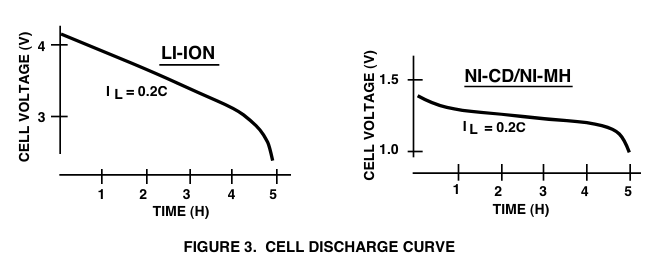
\includegraphics[width=0.7\textwidth]{img/cellDischargeCurve_TxInst.png}
			\caption{Curva de descarga de una celda Li-ion y una celda Ni-Cd/Ni-MH.}
			\label{fig: curva descarga celdas}
		\end{center}
	\end{figure}
	
	\pagebreak 
	
	\noindent \textit{\textbf{Corriente pico}}\\	
	
	\noindent \textit{\textbf{Autodescarga}}\\	
	
	\noindent \textit{\textbf{Tiempo de carga}}\\	
	
	\noindent \textit{\textbf{Coste}}\\
	
	\noindent \textit{\textbf{Fiabilidad}}\\		
	
	\noindent \textit{\textbf{Modos de falla relacionados con la edad}}\\	
	
	\noindent \textit{\textbf{Temperatura de funcionamiento}}\\	
	
	\noindent \textbf{Placa solar}\\ 
	
	\noindent Requieren de una batería donde almacenar la energía que captan/generan, por lo que, necesariamente, habría que escoger entre algunas de las opciones planteadas en el apartado anterior. \\
	
	\noindent \textit{Funcionamiento de un panel solar}
	
	\begin{figure}[h]
		\begin{center}
			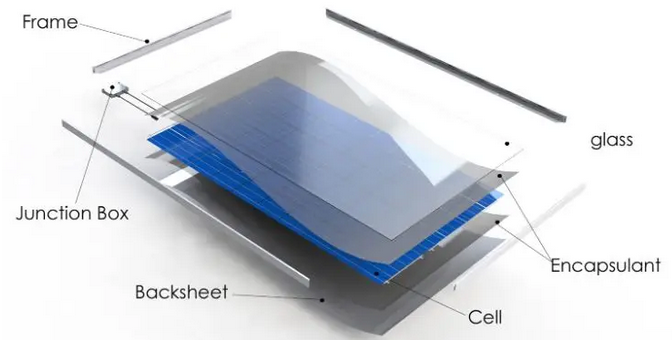
\includegraphics[width=0.6\textwidth]{img/layersSolarPanel.png}
			\caption{Capas y componentes que componen un panel solar.}
			\label{fig: capas panel solar}
		\end{center}
	\end{figure}

	\pagebreak
	
	\noindent Un panel solar es una agrupación de muchas células fotovoltaicas (PV) que están cubiertas con vidrio protector y unidas con un marco de metal. Es por eso que el nombre oficial de un panel solar es "módulo fotovoltaico" (\textit{PV module}). Estas células solares fotovoltaicas están hechas de material semiconductor, generalmente silicio, que se corta en tiras muy finas.\\
	
	\noindent Los paneles solares tienen muchas capas. La capa de células fotovoltaicas es donde se produce la electricidad. Otras capas, como las capas de vidrio y encapsulante, están ahí para proteger las células fotovoltaicas para que los módulos puedan producir electricidad de manera adecuada.\\
	
	\noindent Cada célula fotovoltaica tiene una capa negativa y una capa positiva. La capa negativa tiene electrones adicionales y la capa positiva tiene espacio para esos electrones. La electricidad mueve electrones, por lo que para que un panel solar genere electricidad solo necesitamos algo de energía para hacer que esos electrones se suelten y fluyan de la capa negativa a la capa positiva. \\
	
	\noindent La energía de los fotones del sol suelta los electrones en el lado negativo de la celda fotovoltaica y los hace moverse, lo que significa que ahora tenemos electricidad fluyendo. Esto se llama efecto fotovoltaico.\\
	
	\begin{figure}[h]
		\begin{center}
			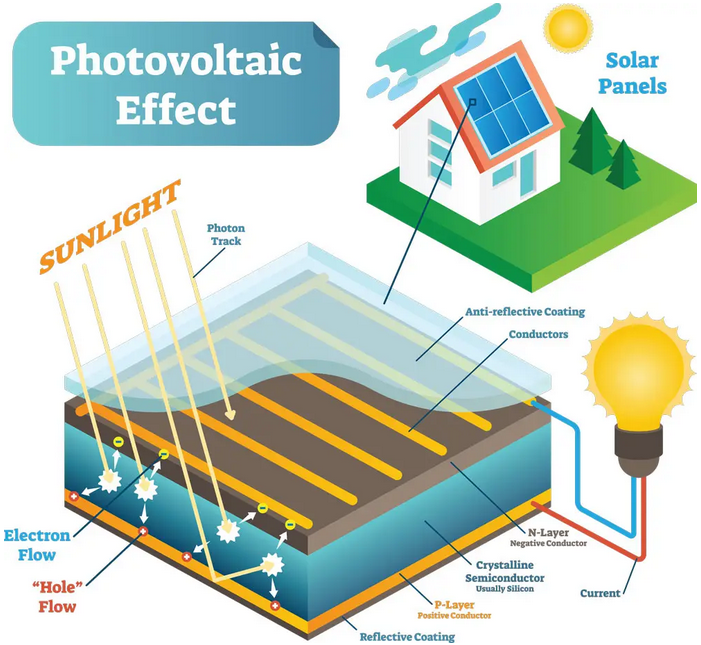
\includegraphics[width=0.6\textwidth]{img/photovoltaic_effect.png}
			\caption{Dibujo representativo del efecto fotovoltaico.}
			\label{fig: efecto fotovoltaico}
		\end{center}
	\end{figure}
	
	\pagebreak
	
	\noindent Los electrones necesitan un camino a seguir y la electricidad debe estar en una forma útil. Es por ello que la ruta que creemos para los electrones (el circuito) es importante, ya que, cuando salen de la capa negativa de la celda fotovoltaica, queremos que fluyan a través de nuestras cargas (como nuestras luces y electrodomésticos, en el ejemplo del uso doméstico) para que los electrones puedan dar energía a esas cargas a medida que avanzan hacia la capa positiva de la celda fotovoltaica. \\
	
	\noindent \textit{\textbf{Uso en hogares de energía solar}} \\
	
	\noindent Los paneles solares producen electricidad de corriente continua (CC, DC), pero la generación de electricidad que usamos en nuestros hogares es de corriente alterna (CA, AC). Para solucionar este problema, agregamos un inversor a nuestro circuito. Luego, el inversor convierte la energía de CC en energía de CA. \\
	
	\noindent El inversor es un factor clave para determinar cómo funcionan los paneles solares porque sin un inversor en nuestro sistema fotovoltaico, no podemos hacer mucho con la energía generada por los paneles solares. Esto último no aplica a nuestro caso, donde nos interesa crear un proyecto que se alimente de manera autónoma, sin uso de la electricidad disponible en el hogar; el panel solar, en este caso, recargaría una pila, y por ello necesitamos la energía DC, y no necesitamos usar un inversor a AC. \\ 
	
	\noindent \textit{Composición de un panel solar} \\
	
	\noindent \textit{Opciones}\\
	
	\noindent \textit{Parámetros}\\
	
	\noindent Los principales paramétros que se usan para caracterizar el rendimiento de las células solares son la potencia máxima $P_{max}$ (\textit{peak power}), la densidad de corriente en cortocircuito $J_{sc}$, la tensión en circuito abierto $V_{oc}$, y el factor de forma \textit{FF}. Estos parámetros se determinan a partir de la curva J-V característica cuando la célula está iluminada, tal como se muestra en la Figura \ref{fig: curva J-V célula solar}. La eficiencia de conversión $\eta$ se puede determinar a partir de estos parámetros. \\
	
	\noindent Nótese que se menciona específicamente \textit{parámetros de una célula solar}; un panel solar, como se ha mencionado anteriormente, consta de varias células fotovoltaicas, por lo que los parámetros especificados, en términos globales y tal como se construyen los paneles solares, influyen en las especificaciones finales del panel según el número de células del que conste. \\
	
	\begin{figure}[h]
		\begin{center}
			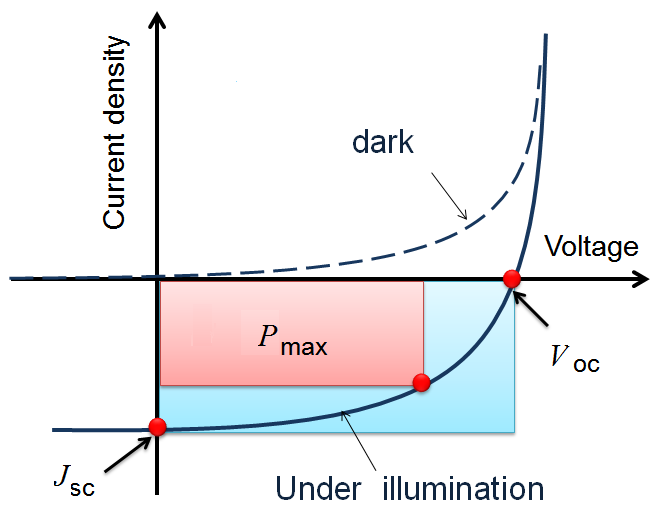
\includegraphics[width=0.5\textwidth]{img/JV_curve_solarCell.png}
			\caption{Determinación de los parámetros de una célula solar a partir de su curva J-V.}
			\label{fig: curva J-V célula solar}
		\end{center}
	\end{figure}
	
	\noindent Para realizar medidas fiables y definir la curva característica J-V, se deben realizar las medidas bajo condiciones estándar de pruebas (\textit{standard test conditions, STC}); estas son, una temperatura constante a $25^{\circ}C$, una irradiancia total de 1000 $W/ m^2$ y un espectro solar de AM1.5 (sol directo y con ángulo cenital de $48,2 ^{\circ}$). Esto lo tendremos en cuenta si queremos comprobar que las especificaciones del producto son correctas, o por el contrario el producto viene defectuoso. En este proyecto no es prioritario el estudio profundo y comprobación exhaustiva del panel solar, por lo que no se realizarán dichas pruebas; sin embargo, sí realizaremos un estudio teórico de los parámetros que definen a una célula solar, como también lo hemos hecho de los materiales que lo componen y su funcionamiento general.\\
	
	\noindent \textit{\textbf{Densidad de corriente en cortocircuito}} \\
	
	\noindent La corriente en cortocircuito $I_{sc}$ es la corriente que fluye a través de un circuito externo cuando los electrodos de una célula solar se cortocircuitan. La corriente en cortocircuito de una célula solar depende de la incidencia del flujo de fotones sobre ella, la cual está determinada por el espectro de la luz incidente. También depende del área de la célula solar. Para eliminar la dependencia del área de la célula solar sobre $I_{sc}$, normalmente se usa la densidad de corriente en cortocircuito para describir la máxima corriente entregada por una célula solar. La máxima corriente que una célula solar puede entregar depende mucho de las propiedades ópticas de la célula solar, tales como la absorción en la capa absorbente y la reflexión. \\
	
	\noindent Las células solares de silicio cristalino pueden entregar, bajo un espectro AM1.5, una posible densidad de corriente máxima de 46 $mA/cm^2$. En las células solares de c-Si de laboratorio, las medidas de $J_{sc}$ están por encima de 42 $mA/cm^2$, mientras que las células solares comerciales tienen un $J_{sc}$ que excede los 35 $mA/cm^2$. \\
	
	\noindent \textit{\textbf{Tensión en circuito abierto}} \\
	
	\noindent La tensión en circuito abierto es la tensión en la cual ninguna corriente fluye a través de un circuito externo. Es la tensión máxima que una célula solar puede entregar. $V_{oc}$ corresponde a la tensión de polarización directa, a la cual la densidad de corriente de oscuridad compensa la densidad de corriente fotovoltaica (\textit{fotocorriente}). Depende de la densidad de corriente de saturación de la célula solar y de la corriente fotogenerada. Mientras ésta última varía poco, la corriente de saturación puede variar en órdenes de magnitud. La corriente de saturacón depende de la recombinación en la célula solar, por lo que $V_{oc}$ es una medida de la cantidad de recombinación de la célula solar.\\
	
	\noindent Las células solares de laboratorio hechas de silicio cristalino dan valores de $V_{oc}$ de hasta 720 mV bajo condiciones AM1.5 estándar, mientras que las células solares comerciales normalmente dan valores de $V_{oc}$ por encima de los 600 mV. \\
	
	\noindent \textit{\textbf{Factor de forma}} \\
	
	\noindent El factor de forma es \\
	
	\noindent \textit{\textbf{Eficiencia de conversión}} \\
	
	\noindent \textit{\textbf{Circuito equivalente}} \\
	
	
%	\noindent Uno de los parámetros más importantes en un panel solar es la \texttt{eficiencia}. Mide el porcentaje de luz solar que llega a la celda solar y que se convierte en electricidad utilizable. Cuanto mayor sea la eficiencia, menor será la superficie que necesitarán los paneles solares para satisfacer sus necesidades energéticas, pero mayor será el precio. \\
	
%	\noindent Algunas personas asocian mayores niveles de eficiencia con paneles de mayor calidad, pero esto no es necesariamente cierto. Alta eficiencia significa que su sistema fotovoltaico solar utilizará menos espacio en su azotea. Por lo tanto, quienes viven en áreas de alta densidad y tienen un espacio muy limitado para la energía solar generalmente están más preocupados por los niveles de eficiencia. \\
	
	\subsubsection{Automatización y monitorización}
	
	\subsubsubsection{Microcontrolador}
	\subsubsubsection{Comunicación radio}
	\subsubsubsection{Comedero}
	\subsubsubsection{Bebedero}
		
	\subsubsection{Prototipo exterior}

	% Definición funcionalidades: qué debo hacer y qué necesitaría
	% Investigación componentes (*) e integración (programación)
		%(*) Qué se ha usado, desglosado por funcionalidades: bebedero, comedero, alimentación, microcontrolador y radio.
		% Descripción, foto, foto en prototipo protoboard
	% Definición prototipo provisional: opciones que he descartado, QR de que funciona?
	% Diseño PCB
	% Desarrollo BBDD en servidor y app web para ver el estado del sistema de alimentación
	
	\subsection[Elección soluciones]{Elección de soluciones para cada funcionalidad}
	
	\subsubsection{Alimentación autónoma del dispositivo}
	\subsubsection{Automatización y monitorización}
	\subsubsubsection{Entorno Arduino}
	
	% Intro: qué es Arduino
	
	Arduino es una plataforma de electrónica \textit{open-source} basada en hardware y software fáciles de usar. Las placas Arduino son capaces de leer entradas (como la luz en un sensor, un dedo pulsando un botón) y convertirlas en salidas (activar un motor, apagar o encender un LED); es decir, como usuarios podemos decirle qué hacer a la placa enviándole una serie de instrucciones al microcontrolador de la placa. Para poder hacer esto último, se hace uso del lenguaje de programación de Arduino (basado en \href{http://wiring.org.co/}{\textit{Wiring}}) y el software de Arduino (IDE, basado en \href{https://processing.org/}{\textit{Processing}}). \\
	
	\noindent A lo largo de los años, Arduino ha sido el corazón de miles de proyectos, desde objetos cotidianos hasta complejos instrumentos científicos. Una comunidad mundial de creadores (estudiantes, aficionados, artistas, programadores y profesionales) se ha reunido en torno a esta plataforma de código abierto, sus contribuciones se han sumado a una increíble cantidad de conocimiento accesible que puede ser de gran ayuda tanto para principiantes como para expertos. \\
	
	\noindent  \textbf{\large Origen} \\ 
	
	\noindent Arduino nació en el Ivrea Interaction Design Institute como una herramienta fácil para la creación rápida de prototipos, dirigida a estudiantes sin experiencia en electrónica y programación. Tan pronto como llegó a una comunidad más amplia, la placa Arduino comenzó a cambiar para adaptarse a las nuevas necesidades y desafíos, diferenciando su oferta desde placas simples de 8 bits hasta productos para aplicaciones de IoT, wearable, impresión 3D y entornos integrados. Todas las placas Arduino son completamente de código abierto, lo que permite a los usuarios construirlas de forma independiente y eventualmente adaptarlas a sus necesidades particulares. El software también es de código abierto y está creciendo gracias a las contribuciones de los usuarios de todo el mundo. \\

	
	\noindent \textbf{\large Características} \\
	
	\noindent La principal característica de Arduino es la simplicidad para trabajar con microcontroladores. A raíz de esto, ofrece una serie de ventajas para sus usuarios, como son:
	\begin{itemize}
		\item \textbf{Es de bajo coste}. Las placas de Arduino son relativamente de bajo coste comparadas con las plataformas de otros microcontroladores. La versión más económica de un módulo Arduino puede ser ensamblada a mano, e incluso los módulos Arduino pre-ensamblados cuestan menos de 50 \$.
		\item \textbf{Multiplataforma}. El software de Arduino, Arduino IDE, es capaz de ejecutarse en Macintosh OSX, Windows y Linux. La mayoría de sistemas de microcontroladores están limitados a Windows.
		\item  	\textbf{Entorno de programación simple y claro}. El software de Arduino (IDE) es fácil de usar para principiantes, sin dejar de ser lo suficientemente flexible para usuarios más avanzados.
		\item \textbf{Software Open Source y extensible}. El software Arduino está publicado como un conjunto de herramientas open source, disponible para ser ampliada por otros programadores a través de librerías basadas en el lenguaje C++; las personas que quieran comprender los detalles técnicos pueden dar el salto de Arduino al lenguaje de programación AVR C en el que se basa. Del mismo modo, se puede agregar código AVR-C directamente en los  programas Arduino si así se desea.
		\item \textbf{Hardware Open Source y extensible}. Los planos de las placas Arduino están publicados bajo licencia \textit{Creative Commons}, así pues, diseñadores de circuitos experimentados pueden hacer su propia versión del módulo, extendiéndola y mejorándola. Incluso usuarios sin experiencia pueden crear una versión en protoboard del módulo para entender cómo funciona y ahorrar dinero.
	
	\end{itemize}

	\noindent \textbf{\large Hardware: placas Arduino} \\
	
	\noindent Existen diferentes placas Arduino, cuya elección dependerá del objetivo que persiga nuestro proyecto y de los requerimientos y limitaciones sobre dicho proyecto. \\
	% Electrónica: arduino nano
	
	\noindent \textbf{\large Software: Arduino IDE}
	
	% Programación: arduinoIDE, void loop y setup, define, etc
	
	\subsubsubsection{LoRa}
	
	\noindent \textbf{Qué es}\\
	
	\noindent El término LoRa proviene de la unión de las palabras \textit{Long} y \textit{Range}, es decir, largo alcance, evidenciando, así, a través de su nombre una de sus principales características. Se trata de la capa física del protocolo \textit{LoRaWAN}; es a través de esta capa que se permite el establecimiento del enlace de comunicación de largo alcance, mientras que LoRaWAN define el protocolo de comunicación y la arquitectura del sistema para la red. \\
	
	\noindent También se trata de una tecnología inalámbrica propiamente dicha que ofrece una transmisión de largo alcance, bajo consumo y segura para aplicaciones IoT y M2M. Se basa en la modulación de espectro ensanchado, la cual presenta características de bajo consumo como la modulación FSK pero puede ser usada para comunicaciones de largo alcance. Puede ser usada para conectar sensores, gateways, máquinas, dispositivos, animales, personas, etc. de manera inalámbrica a la nube.\\
	
	\noindent \textbf{Planes de frecuencia} \\
	
	\noindent La tecnología LoRa opera en diferentes frecuencias dependiendo de la región en la que nos encontremos, por ejemplo: \\
	
	\begin{itemize}
		\item En Norteamérica, opera en la banda de 915 MHz.
		\item En Europa, en la banda de 868 MHz.
		\item En Asia, en la banda de 865 a 867 MHz y en la banda 920 a 923 MHz, aunque es común también la banda 433 MHz.
	\end{itemize}
	
	\noindent Dado que los planes de frecuencia para LoRa varían según la región, inclusive país, es recomendable asegurarse de las regulaciones vigentes en cada país para el uso del espacio radioeléctrico. A modo resumen y como orientación inicial a este asunto, se puede consultar esta \href{https://www.thethingsnetwork.org/docs/lorawan/frequencies-by-country/index.html}{lista de planes de frecuencia para cada país}, elaborada por \textit{The Things Network}. \\
	
	\noindent \textbf{Origen} \\
	
	\noindent La tecnología LoRa fue creada por una compañía francesa llamada \textit{Cycleo}, la cual posteriormente fue adquirida por Semtech en 2012. Semtech fue el miembro fundador de \textit{LoRa Alliance}, que actualmente es el organismo rector de LoRa Technology. LoRa Alliance es una de las alianzas tecnológicas de más rápido crecimiento. Esta asociación sin ánimo de lucro está formada por más de 500 empresas miembro, comprometidas a permitir la implementación a gran escala de redes IoT de amplia cobertura y baja potencia (LPWAN) a través del desarrollo y la promoción del estándar abierto LoRaWAN.\\
	
	\noindent \textbf{Especificaciones en términos generales de la tecnología LoRa}
	
	\begin{itemize}
		\item Órgano rector: LoRa Alliance
		\item Estándar: 801.15.4g
		\item Frecuencia: banda ISM, 868/916 MHz
		\item Alcance: hasta 5 km (urbano) y hasta 15 km (rural)
		\item Datarate: 27 kbps
		\item Modulación: espectro ensanchado basado en la tecnología de modulación FM
		\item Seguridad: CRC de 32 bits
	\end{itemize}
	 
	 %LoRaWAN is a Low Power, Wide Area (LPWA) networking protocol developed by the LoRa Alliance, that wirelessly connects battery operated ‘things’ to the internet in regional, national or global networks, targeting key Internet of Things (IoT) requirements such as bi-directional communication, end-to-end security, mobility and localization services.
	 
	% LoRaWAN uses unlicensed spectrum in the ISM bands to define the communication protocol and system architecture for the network while the LoRa physical layer creates the long-range communication links between remote sensors and gateways connected to the network. This protocol helps in the quick setup of public or private IoT networks anywhere using hardware and software.
	
	\noindent  \textbf{Regulación LoRa en Europa: ERC 70-03} \\
	
	\noindent \href{https://docdb.cept.org/download/25c41779-cd6e/Rec7003e.pdf}{ERC 70-03} \\
	
	%% CAPA FISICA DE LORAWAN %%
	
	\pagebreak
	
	\subsubsubsection{LoRaWAN: NO VA AQUÍ, VA EN APARTADO 3.2}
	
	\noindent A pesar de que no se va a usar LoRaWAN en este proyecto, sí que se realizó su pertinente investigación, por lo que a continuación se muestra un resumen de nociones básicas sobre LoRaWAN. \\
	
	\noindent \textbf{Clases de nodos finales LoRaWAN}  \\
	
	\noindent Existe 3 clases diferentes de nodos finales en LoRaWAN, los cuales son:
	
	\begin{itemize}
		\item Clase A (\textit{All})
		\item Clase B (\textit{Beacon})
		\item Clase C (\textit{Continuous})
	\end{itemize}
	
		\begin{figure}[h]
		\begin{center}
			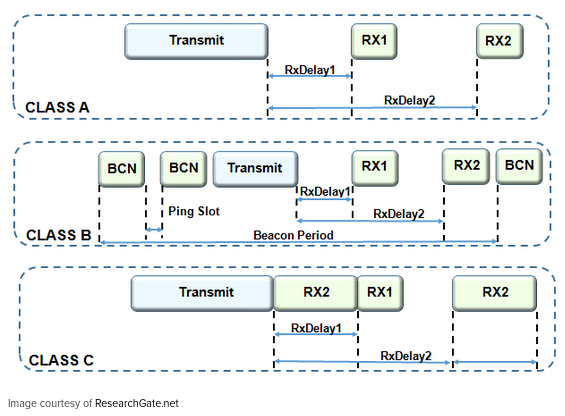
\includegraphics[width=0.7\textwidth]{img/endDevices.png}
			\caption{Funcionamiento de nodos finales usando LoRaWAN.}
		\end{center}
	\end{figure}
	
	\pagebreak
	
	\noindent \textbf{Estructura de un paquete LoRaWAN}
	
	\begin{figure}[h]
	\begin{center}
			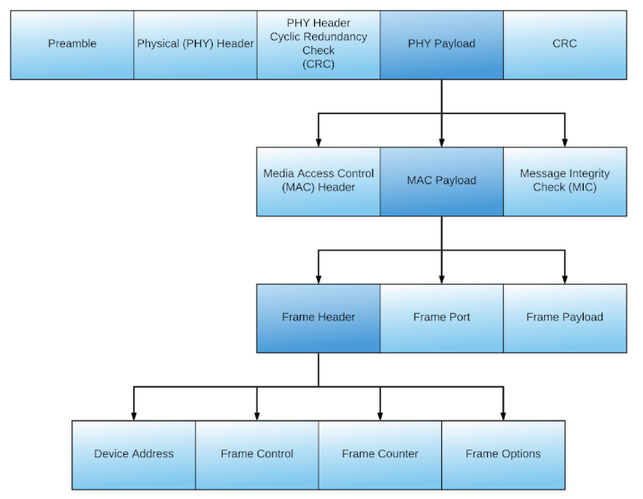
\includegraphics[width=0.7\textwidth]{img/lora_phyLayer_packetFormat.png}
			\caption{Estructura general de un paquete LoRaWAN.}
	\end{center}
	\end{figure}
	

	
	\begin{figure}[h]
	\begin{center}
			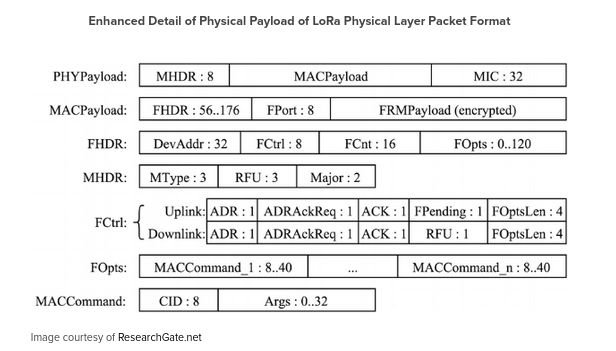
\includegraphics[width=0.7\textwidth]{img/lora_phyLayer_packetFormat_enh.png}
			\caption{Estructura detallada de un paquete LoRaWAN.}
	\end{center}
	\end{figure}

	\pagebreak

%	\subsection[Monitorización y automatización]{Monitorización y automatización}
	
%	El Arduino que vamos a usar es el Arduino nano, como ya se ha comentado anteriormente. Los sensores que vamos a usar son:
	
%	\pagebreak
%	\subsection[Comunicaciones LoRa]{Comunicaciones LoRa}

%	Los módulos LoRa que vamos a usar son los E32-868T30D (como ya se ha comentado anteriormente).
%	\subsubsection{Cálculo teórico de pérdidas de enlace}
%	\subsubsection{Simulación en \textit{Radio Mobile}}
	
%	\subsection{Alimentación del dispositivo}

	\subsubsubsection{Comedero}
	
	\subsubsubsection{Bebedero}
	
	\subsubsection{Prototipo exterior}
		
	\subsection[Resumen del capítulo]{Resumen de capítulo}
	
	En este capítulo se ha hablado de las dos principales tecnologías usadas en este proyecto. Se han explicado de forma teórica, después se ha explicado cómo se integran en el proyecto en la parte de monitorización y automatización en el caso de Arduino, y en la parte radio en el caso de LoRa. Se hace un acercamiento a software de simulación radio. Se sacan conclusiones para la creación de un prototipo que pueda ser ejecutado y probado en el entorno objetivo.
	\pagebreak
	
	
	\section[Prototipo y pruebas]{Prototipo y pruebas}
	
	% Ensamblado PCB y pruebas
	\subsection[Ubicación]{Ubicación}
	\subsection[Prototipo inicial]{Prototipo inicial}
	\subsection[Prototipo definitivo]{Prototipo definitivo}
	\subsection[Pruebas]{Pruebas}
	\subsection[Comentarios sobre los resultados de las pruebas]{Comentarios sobre los resultados de las pruebas}
	\subsection[Presupuesto]{Presupuesto}
	\noindent Se adjunta una tabla para el desglose del presupuesto para este proyecto en el Anexo III (\ref{subsection: presupuesto}).
	\subsection[Resumen del capítulo]{Resumen del capítulo}
	
	\section[Conclusiones y líneas futuras]{Conclusiones y líneas futuras}
	
	\section*{Glosario}
	\addcontentsline{toc}{section}{Glosario}
	
	\section*{Bibliografía}
	\addcontentsline{toc}{section}{Bibliografía}
	
	\section*{Anexos}
	\addcontentsline{toc}{section}{Anexos}
	
	\subsection*{Anexo I}
	\addcontentsline{toc}{subsection}{Anexo I}	
	
	\subsection*{Anexo II}
	\addcontentsline{toc}{subsection}{Anexo II}
	
	\subsection*{Anexo III}
	\label{subsection: presupuesto}
	\addcontentsline{toc}{subsection}{Anexo III}
	
	
\end{document}